\chapter{The Models}

\section{Solver and Critic}
% Gemma and Qwen sources, versions, and characteristics.

\section{Rationale for Using Different Models}
% Jafari's suggestion, reduced automatic agreement, and downstream effects.

\section{Sparse Autoencoder Sources}

The experiments use two principal SAE sources: a pretrained JumpReLU SAE from
Gemma Scope and custom SAEs trained on activations from the Solver--Critic
pipeline. Keeping both sources provides a useful comparison. The pretrained
SAE represents a general-purpose dictionary learned independently of the
feedback-uptake labels, whereas the custom SAEs are matched to the activation
distribution produced by this study. We additionally evaluated adapted copies
of the pretrained SAE in which selected parameters were updated on the
interaction data. These adapted models are treated as separate experimental
representations rather than as replacements for the original checkpoint.

\subsection{Pretrained Gemma Scope SAE}

The pretrained representation is a Gemma Scope 2 JumpReLU SAE compatible with
the Gemma 3 4B instruction-tuned Solver \cite{lieberum2024gemmascope}. We use
the residual-post SAE attached to the output of transformer layer 25. Its
dictionary contains 16,384 features and has a nominal $L_0$ target of 120
active features per activation. The checkpoint is identified in the repository
as \texttt{layer\_25\_width\_16k\_l0\_big}; its model configuration records
the hook point as \texttt{model.layers.25.output} and the source model as
\texttt{google/gemma-3-4b-it}.

JumpReLU applies a learned threshold to each encoder preactivation. Features
below their thresholds are set to zero; features above threshold retain a
continuous magnitude. The pretrained checkpoint is used without updating its
parameters in the primary pretrained-SAE comparison. This preserves the
dictionary as an external baseline and avoids using the feedback-uptake labels
to construct its feature basis.

We also created a decoder-adapted variant to test whether reconstruction on the
project's activation distribution could be improved while preserving the
pretrained feature detector. In this variant, the JumpReLU encoder and
thresholds remain fixed and only the decoder-side reconstruction is fitted to
the interaction activations. Because the encoder is unchanged, the original
and adapted variants produce the same latent activations and feature rankings;
they differ only in how a latent edit is mapped back into the Solver's residual
stream. This distinction is important when interpreting causal results: a
change in steering behavior can arise from the decoder geometry even when the
selected feature activations are identical.

\subsection{Custom Interaction-Trained SAEs}

The custom SAEs are trained from scratch on Layer 25 residual-post activations
collected during the Solver's second turn. Each input is a
2,560-dimensional residual vector from the last prompt token. The dictionary
contains 12,888 latent features, making it approximately five times wider than
the input representation. Only training-partition activations are used to fit
the parameters. Validation activations are used for model selection, while
held-out partitions are reserved for downstream evaluation and intervention.

Before training, activations are divided by a single root-mean-square scale
computed over all elements of the training activations. The same scale is
reused for every split, and decoder outputs are multiplied by it to return to
the Solver's original activation units. Decoder columns are initialized with
unit $L_2$ norm and renormalized after each optimization step. The models use
tied encoder--decoder initialization, seed 42, shuffled batches of 256, a
maximum of 200 epochs, and early stopping after 20 epochs without a sufficiently
large validation improvement.

We trained two custom sparsity strategies because they impose different
representation tradeoffs:

\begin{itemize}
    \item \textbf{$L_1$ SAE.} Nonnegative latent activations are penalized by
    an $L_1$ term with coefficient 2.0. The selected model uses a learning rate
    of $10^{-4}$. Its objective is reconstruction mean-squared error plus the
    weighted mean absolute latent activation.

    \item \textbf{TopK+AuxK SAE.} For each example, the main path retains the
    128 largest nonnegative encoder activations. The selected model uses a
    learning rate of $3\times10^{-4}$. An AuxK reconstruction term with
    coefficient $1/128$ and up to 512 eligible inactive features provides a
    training signal to features that are not selected by the main TopK path
    \cite{gao2025scaling}. The auxiliary loss is used only during training;
    validation selection uses the main-path reconstruction loss.
\end{itemize}

The two strategies were selected from validation sweeps rather than by choosing
the lowest reconstruction error alone. We considered reconstruction
mean-squared error, variance explained, the number of active features per
example, and the proportion of the dictionary that fired at least once. As
Figure~\ref{fig:sae-selection-rationale} summarizes, TopK+AuxK provided stronger
reconstruction at exactly 128 active features per example but used a relatively
small portion of the full dictionary. The $L_1$ model accepted higher
reconstruction error in exchange for fewer active features per example and
broader dictionary coverage. This comparison was used to characterize the
custom SAE design space; it did not mean that both custom models entered the
final downstream experiments. The TopK+AuxK model was excluded from final
downstream tasking. Those analyses used the $L_1$ custom SAE and the pretrained
SAE family, including its adapted variants.

\begin{figure}[htbp]
    \centering
    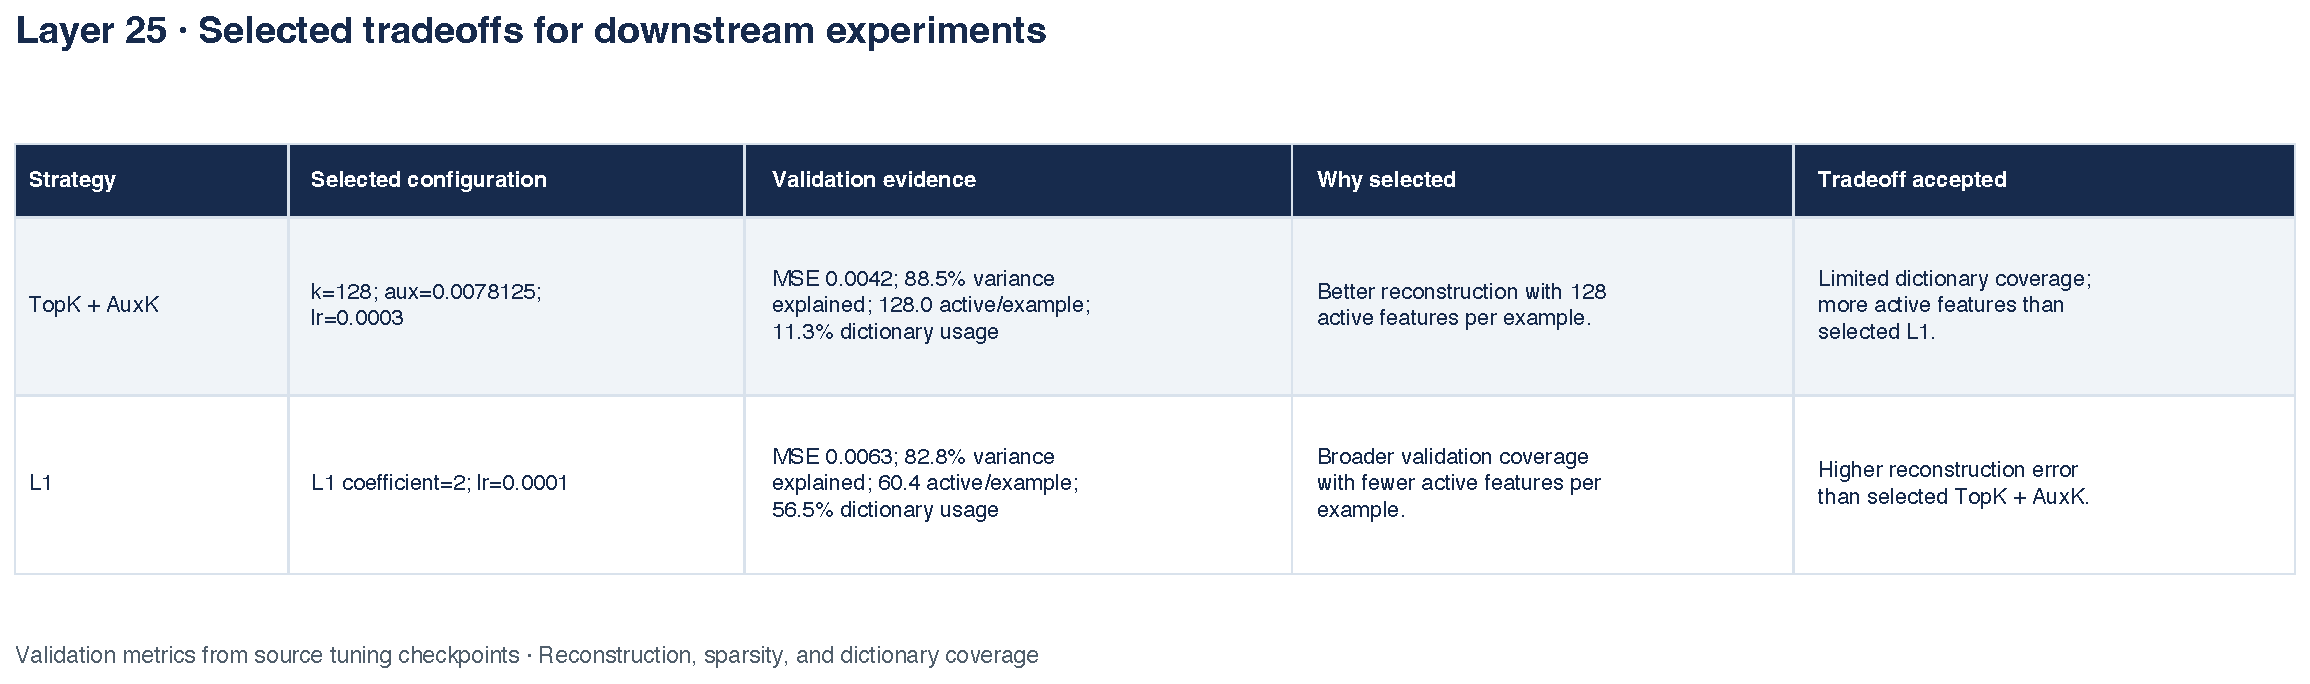
\includegraphics[width=\textwidth]{build_figures/sae_selection_rationale.pdf}
    \caption{Validation tradeoffs used to select the Layer 25 custom SAEs. The
    TopK+AuxK checkpoint prioritizes reconstruction with a fixed activity
    budget, whereas the $L_1$ checkpoint provides broader dictionary coverage
    with fewer active features per example. Metrics are computed from the
    source tuning checkpoints on held-out validation activations.}
    \label{fig:sae-selection-rationale}
\end{figure}

\clearpage
\section{Model Limitations}

The model choices make the experiments feasible and reproducible, but they
also limit the scope of the conclusions. First, both the Solver and Critic are
approximately four-billion-parameter instruction-tuned models. Their behavior
may differ from substantially larger frontier models, smaller local models, or
models trained with different instruction and alignment procedures. Results
from the Gemma--Qwen pairing should therefore be interpreted as evidence about
one controlled multi-model system rather than a universal account of feedback
uptake.

Second, the mechanistic analysis focuses on one Solver family and ultimately
one residual-stream site: the output of Layer 25 at the final prompt token.
This design was necessary because collecting activations, training several
wide SAEs, and replaying hundreds of intervention conditions are expensive.
It does not establish that the same features exist at other layers, that Layer
25 is the only location where uptake is represented, or that the last-token
state captures the full temporal process by which feedback is evaluated.

Third, every SAE is an imperfect transformation of the Solver activation. The
custom dictionaries have finite width and incomplete feature utilization, and
the pretrained Gemma Scope SAE was trained on a broader distribution than the
project's candidate-presentation prompts. Passing an activation through an SAE
can therefore change the model even when no feature is intentionally edited.
The reconstruction-control experiments measure this effect, but they cannot
guarantee that every intervention remains on the natural activation manifold.
Likewise, a sparse or causally effective latent is not automatically
monosemantic or human-interpretable.

Fourth, compute constraints limited hyperparameter searches, independent
training seeds, and replication across model sizes and datasets. The custom
SAE sweep compares two principal sparsity mechanisms at a fixed dictionary
width and uses seed 42; it is not an exhaustive comparison of SAE
architectures. Some checkpoints and activation tensors are also too large to
store directly in the Git repository and must be retrieved from the project's
artifact storage. Reproduction consequently depends on access to the named
model weights, compatible hardware, and the archived checkpoints.

Finally, deterministic decoding improves replay consistency but narrows the
behavioral distribution. The findings describe how these particular models
respond under the fixed prompts, candidate-presentation format, decoding
settings, and MuSiQue-derived task distribution. Generalization to free-form
dialogue, stochastic sampling, longer feedback exchanges, other domains, or
human-provided criticism remains an open question.
